\chapter{Sicurezza}

\section{Autenticazione}
L'autenticazione  mediante SSO di ogni applicazione richiede una serie di scambi tra l'applicazione stessa e Cas che sono rappresentati nel grafico seguente e descritti poco dopo:

\begin{figure}[h!]
  \centering
    \includegraphics[scale=0.8]{disegno} 
  \caption[cas]{Processo di autenticazione \label{fig:cas}}
\end{figure}

\begin{enumerate*}
\item Quando un browser tenta di accedere per la prima volta ad un'applicazione (d'ora in poi Client) realizzata con Regola kit e protetta con cas il browser viene reindirizzato all'applicazione Cas (d'ora in poi CAS) passandole come parametro una stringa che rappresenta il servizio richiesto. Su CAS attraverso un form HTML l'utente inserisce username e password. A questo punto, se l'autenticazione è andata a buon fine, CAS conosce il netID dell'utente autenticato, ad esempio nicola.santi@unibo.it

\item  CAS ridirige il browser all'applicazione Client passandole come parametro il service ticket, un numero che servirà poi in seguito.

\item  Client richiama CAS passandogli il service ticket appena ricevuto ed una URL chiamata pgt url che CAS userà in seguito. A questa chiamata CAS risponde con il netID dell'utente (nicola.santi@unibo.it) ed un altra stringa, il pgtIOU che servirà in seguito.

\item  CAS richiama il client alla url che aveva ricevuto nella richiesta precedente (la pgt url) ed invia a Client di nuovo lo stesso pgtIOU di prima perché Client verifichi che siano uguali ed inoltre invia un pgt da usare in seguito nell'autenticazione di tipo proxy.

A questo punto l'autenticazione di un utente che voleva accedere a Client tramite browser è terminata. Rimane da spiegare l'autenticazione di tipo proxy, ovvero se Client decide di invocare ad esempio un servizio web di un'altra applicazione, diciamo Server senza doversi riautenticare.

\item Client invia il pgt a CAS che gli risponde con il proxy ticket, una stringa da passare a Server.

\item Client richiama Server e gli passa il proxy ticket.

\item Server contatta CAS passandogli il proxy ticket e la pgt url. A questa chiamata CAS risponde con il netID dell'utente (nicola.santi@unibo.it) ed un altra stringa, il pgtIOU che servirà in seguito. Questo passaggio è del tutto simile a quello numero 3. Seguirà una passaggio simile a 4 in cui CAS chiamerà Server passandogli pgt e pgtIOU.
\end{enumerate*}

Le url coinvolte nei passaggi precedenti sono configurabili all'interno dell'applicazione Client modificando alcune proprietà nel file  src/main/webapp/WEB-INF/cas.properties. La tabella seguente riporta le url coinvolte per ogni passo unitamente alla proprietà da configurarare ed il suo valore di default:

\begin{center}
  \begin{tabular}{ | l | l | l |}
  \hline
  step  &  URL    & parametro \\ \hline
  1  &  login url &  cas.loginUrl=/login \\ \hline
  2  &  service url &  cas.main=/personale/j\_acegi\_cas\_security\_check \\ \hline
  3,7 & validation url &   cas.validationUrl=/proxyValidate\\ \hline
  4 & pgt url  & cas.pgtUrl=/casProxy  \\ \hline
  5 &  proxy url &  cas.proxyUrl=/proxy \\ \hline
  6 & la url specifica del servizio &  \\ \hline
  \end{tabular}
\end{center}


\section{Configurazione di Cas}
Affinché la propria applicazione (Client o Server) possa usufruire del SSO deve registrare presso Cas uno (o più servizi). I servizi sono essenzialmente identificati da una stringa che deve corrispondere (anche solo parzialmente come vedremo) con la service url richiamata da Cas al punto 2. Per non restare nel vago immaginiamo di dover registrare un servizio per un'applicazione che risponde alla url https://tirocini.unibo.it e la cui service url sia https://tirocini.unibo.it/j\_acegi\_cas\_security\_check. Il nome del servizio può coincidere con questa url oppure con una suo sottoparte come ad esempio https://tirocini.unibo.it/* (si prega di notare l'asterisco).

Si rammenta che nel caso di autorizzazione di tipo proxy è necessario utilizzare due servizi distinti, uno per l'autenticare l'applicazione Client da passare nel passo 1 ed quello da utilizzare per l'applicazione Server per il passo 5; da notare che il secondo servizio deve coincidere (anche solo parzialmente) con la url di Server mentre il primo con la url di Client.

\section{Configurazione di Client}
Nonostante le possibilità di Cas siano particolarmente ampie, la configurazione di default realizzata da Regola kit dovrebbe soddisfare le esigenze più comuni di un'applicazione web. In questo caso la configurazione si limita a modificare il nome del servizio e l'host dove risponde Cas all'interno del file src/main/webapp/WEB-INF/cas.properties.

\begin{xml}
# servizi registrati per questa applicazione (da riportare sul server CAS) 
cas.service.proxied=/services/
cas.main=/personale/j_acegi_cas_security_check

# url di test
cas.hostUrl=https://localhost:8443/cas
cas.ourAppUrl=https://localhost:8443/${artifactId}

# url di produzione
prod.cas.host=https://localhost:8443/cas
prod.cas.ourAppUrl=https://localhost:8443/${artifactId}
\end{xml}


Nell'esempio abbiamo configurato due servizi, uno per l'autenticazione di tipo proxy ovvero quando la nostra applicazione funziona come Server alla url /services e l'altra per quando l'applicazione nostra funziona come Client. In questo caso conviene usare come nome del servizio la nostra service url, come nell'esempio. Le altre proprietà specificano le url della nostra applicazione e del server Cas sia in produzione sia in test.

La prossima configurazione da modificare si trova del file  src/main/webapp/WEB-INF/security-cas.xml e prevede l'impostazione delle url da proteggere e per ciascuna di esse quale gruppo a titolo per visualizzarle.

\begin{xml}
  <bean id="filterChainProxy" class="org.acegisecurity.util.FilterChainProxy">
    <property name="filterInvocationDefinitionSource">
      <value>
        CONVERT_URL_TO_LOWERCASE_BEFORE_COMPARISON
        PATTERN_TYPE_APACHE_ANT 
        /images/**=#NONE#
        /scripts/**=#NONE# 
        /styles/**=#NONE#
        /portal.jsp=httpSessionContextIntegrationFilter,logoutFilterMain,casProcessingFilter,securityContextHolderAwareRequestFilter,anonymousProcessingFilter,exceptionTranslationFilter,filterInvocationInterceptor
        /personale/**=httpSessionContextIntegrationFilter,logoutFilterMain,casProcessingFilterForMain,securityContextHolderAwareRequestFilter,anonymousProcessingFilter,exceptionTranslationFilterMain,filterInvocationInterceptor
      </value>
      <!--
        Put channelProcessingFilter before
        securityContextHolderAwareRequestFilter to turn on SSL switching
      -->
    </property>
  </bean>
  
  <!-- specifica ruoli che possono accedere alle diverse url  -->
  <bean id="filterInvocationInterceptor"
    class="org.acegisecurity.intercept.web.FilterSecurityInterceptor">
    <property name="authenticationManager" ref="casAuthenticationManager" />
    <property name="accessDecisionManager" ref="accessDecisionManager" />
    <property name="objectDefinitionSource">
      <value>
        PATTERN_TYPE_APACHE_ANT
        /portal.jsp=admin,user
        /esterni/richiesta*.*=ROLE_ANONYMOUS,admin,user
        /esterni/loginMigrazione.*=ROLE_ANONYMOUS,admin,user
        /**/*.htm*=admin,user
        /**/*.jsp*=admin,user
      </value>
    </property>
  </bean>

\end{xml}

Questo è quanto occorre generalmente per consentire alla propria applicazione di funzionare sia come Client che come Server. Nel resto di questo capitolo mostreremo le altre possibili variazioni che comprendono la modifica del file  src/main/webapp/WEB-INF/security-cas.xml ma richiedono una conoscenza più approfondita di Cas e Acegi Securty.


\section{Presentazione}

Il sistema di sicurezza è costruito attorno ad una catena di oggetti chiamati filtri che vengono eseguiti in cascata e cooperano per assolvere i diversi compiti nei quali la funzione della sicurezza si concretizza. Esistono molti filtri standard ma è comunque possibile aggiungerne di personalizzati ad esempio per aggiungere un sistema di autenticazione proprietario o non ancora implementato. L'elenco che segue indica i filtri standard nell'ordine con cui sono eseguiti e per ciascuno il nome della classe che lo implementa ed  un alias per riferirsi ad esso:

\begin{tabular}{ | l | l | }
  \hline
  CHANNEL\_FILTER & ChannelProcessingFilter \\ \hline
  CONCURRENT\_SESSION\_FILTER  & ConcurrentSessionFilter \\ \hline
  SESSION\_CONTEXT\_INTEGRATION\_FILTER  & HttpSessionContextIntegrationFilter  \\ \hline
  LOGOUT\_FILTER & LogoutFilter  \\ \hline
  X509\_FILTER X509 & PreAuthenticatedProcessigFilter \\ \hline
  PRE\_AUTH\_FILTER & Subclass of AstractPreAuthenticatedProcessingFilter\\ \hline
  CAS\_PROCESSING\_FILTER & CasProcessingFilter \\ \hline
  AUTHENTICATION\_PROCESSING\_FILTER & AuthenticationProcessingFilter \\ \hline
  BASIC\_PROCESSING\_FILTER & BasicProcessingFilter \\ \hline
  SERVLET\_API\_SUPPORT\_FILTER & classname \\ \hline
  REMEMBER\_ME\_FILTER & RememberMeProcessingFilter \\ \hline
  ANONYMOUS\_FILTER & AnonymousProcessingFilter \\ \hline
  EXCEPTION\_TRANSLATION\_FILTER & ExceptionTranslationFilter \\ \hline 
  NTLM\_FILTER & NtlmProcessingFilter \\ \hline
  FILTER\_SECURITY\_INTERCEPTOR & FilterSecurityInterceptor \\ \hline
  SWITCH\_USER\_FILTER & SwitchUserProcessingFilter \\ \hline
\end{tabular}

Prima di calarci nel dettaglio dei filtri più importanti conviene concentrarci sulla configurazione più importante del sistema, ovvero quella che specifica quali di questi filtri utilizzare per una certa url e che si concretizza nella definizione del bean filterChainProxy:  


\begin{xml}
<bean id="filterChainProxy"
     class="org.acegisecurity.util.FilterChainProxy">
  <property name="filterInvocationDefinitionSource">
     <value>
    CONVERT_URL_TO_LOWERCASE_BEFORE_COMPARISON
    PATTERN_TYPE_APACHE_ANT 
    /images/**=#NONE#
    /scripts/**=#NONE# 
    /styles/**=#NONE#
    /**=httpSessionContextIntegrationFilter,logoutFilter,authenticationProcessingFilter,securityContextHolderAwareRequestFilter,anonymousProcessingFilter,exceptionTranslationFilter,filterInvocationInterceptor
    </value>
  </property>
</bean>
\end{xml}

L'aspetto è piuttosto intimidatorio sulle prime ma in effetti si limita a specificare le catene di filtri da adottare per le url indicate, nell'esempio dispone di non utilizzare nessun filtro (\#NONE\#) per le url /images/**, /scripts/**, e /style/**. Per tutte le altre url (/**) invece si utilizza la catena dei sette filtri specificati. Si può notare che le url sono indicate utilizzando la notazione di ANT essendo stato passato il parametro   PATTERN\_TYPE\_APACHE\_ANT, alternativamente si potevano utilizzare le espressioni regolari. 
Come si diceva ogni filtro assolve un compito specifico e deve essere configurato per modificarne comportamento; ad esempio l'ultimo dei sette filtri specificati nella catena,  filterInvocationInterceptor, si occupa di stabilire quali utenti (o quali gruppi di utenti) possano accedere alle pagine protette. Si può configurare come segue:

\begin{xml}
<bean id="filterInvocationInterceptor"
  class="org.acegisecurity.intercept.web.FilterSecurityInterceptor">
  <property name="authenticationManager"
 
                  ref="authenticationManager" />
  <property name="accessDecisionManager"
        ref="accessDecisionManager" />
  <property name="objectDefinitionSource">
    <value>
    PATTERN_TYPE_APACHE_ANT
    /services/*=ROLE_ANONYMOUS,admin,user
    /login.*=ROLE_ANONYMOUS,admin,user
    /**/*.html*=admin,user
    </value>
  </property>
</bean>
\end{xml}

Iniziamo dalla proprietà dal nome oscuro  objectDefinitionSource che specifica una serie di url (sempre nel formato ANT) e per ciascuno quale utente o ruolo ha il permesso di accesso; ad esempio le url del tipo /services/* possono essere accedute da tutti (utenti anonimi cioè quelli con il ruolo ROLE\_ANONYMOUS, l'utente admin e l'utente user). Stessa cosa per la pagina di login mentre per tutte le altre pagine l'accesso è consentito solo agli utenti user ed admin. Da notare come queste regole siano applicate in cascata, così come quelle specificate nella configurazione della catena dei filtri. 
Come spesso accade la configurazione di un bean ne richiede altri, nel caso di   filterInvocationInterceptor si utilizzano anche i bean  authenticationManager e  accessDecisionManager. Trattiamo prima quest'ultimo che ha il compito di stabilire  se un utente possa o meno accedere; di solito si utilizza una configurazione standard per in base al ruolo si può accedere o meno. La configurazione è la seguente.

\begin{xml}
<bean id="accessDecisionManager"
  class="org.acegisecurity.vote.AffirmativeBased">
  <property name="allowIfAllAbstainDecisions" value="false" />
  <property name="decisionVoters">
    <list>
      <bean class="org.acegisecurity.vote.RoleVoter">
        <property name="rolePrefix" value="" />
      </bean>
    </list>
  </property>
</bean>
\end{xml}

L'altro bean utilizzato per configurare  filterInvocationInterceptor è  authenticationManager, si tratta di un bean importantissimo che è utilizzato anche da altri filtri (ad esempio  authenticationProcessingFilter, il terzo filtro della catena di sette configurata sopra). Il bean  authenticationManager si occupa infatti di fornire i componenti che effettuano l'autenticazione dell' utente corrente (ad esempio ma non necessariamente utilizzando username e password) e fornire l'oggetto che rappresenta quell'utente ed i ruoli ricoperti all'interno del sistema di sicurezza. Ora, dal momento che i metodi per autenticare un utente potrebbero essere diversi, ad esempio prima su una database poi in caso di fallimento su un altro poi in caso di fallimento tramite LDAP e così via  authenticationManager contiene la lista di questi servizi di autenticazione chiamati authentication provider:

\begin{xml}
<bean id="authenticationManager"
  class="org.acegisecurity.providers.ProviderManager">
  <property name="providers">
    <list>
       <ref local="daoAuthenticationProvider" />
       <ref local="anonymousAuthenticationProvider" />
       <ref local="rememberMeAuthenticationProvider" />
    </list>
  </property>
</bean>
\end{xml}

Come si può immaginare esistono già pronti per l'uso diversi authentication provider come l' anonymousAuthenticationProvider che provvede le credenziali per l'utente anonimo, la cui configurazione si limita a dare un nome (anonymous)  a questo particolare utente.

\begin{xml}
<bean id="anonymousAuthenticationProvider"
    class="org.acegisecurity.providers.anonymous.AnonymousAuthenticationProvider">
  <property name="key" value="anonymous" />
</bean>
\end{xml}

Invece l' authentication provider  rememberMeAuthenticationProvider si occupa di autenticare un utente in base ad un cookie precedentemente salvato sul browser, la cui configurazione (riutilizzando l'uthenticationManager ) non è riportata di seguito per evitare di perdere il filo del discorso.
Ci occupiamo invece del  daoAuthenticationProvider  perché ricopre un ruolo di rilievo nel sistema di sicurezza. Infatti la classe  DaoAuthenticationProvider è in grado di utilizzare tutti i meccanismi di autenticazioni basati su username e password forniti col sistema semplicemente delegando l'individuazione dell'utente e del ruolo ad un bean chiamato userDetailsService.

\begin{xml}
<bean id="daoAuthenticationProvider"
  class="org.springframework.security.providers.dao.DaoAuthenticationProvider">
  <property name="userDetailsService" ref="inMemoryDaoImpl"/>
  <property name="saltSource" ref="saltSource"/>
  <property name="passwordEncoder" ref="passwordEncoder"/>
</bean>    
\end{xml}
  
Nell'esempio lo userDetailsService utitlizzato è inMemoryDaoImpl che si limita a leggere utenti e password direttamente dal file di configurazione.

\section{Configurazione semplificata}

Nel paragrafo precedente abbiamo specificato la catena dei filtri da applicare per ogni url e poi indicato per ogni url quale utente o gruppo pottesse accedere. Infine abbiamo fornito un semplice sistema di autenticazione basato su un file di configurazione di utenti, gruppi e password. In molti hanno pensato che, per quanto flessibile, il sistema di configurazione sopra descritto risulti davvero complicato e finalmente nella versione 2.0 (oltre al cambio di nome da Acegi a Spring Security) è stato introdotto un sistema di configurazione basato su configurazioni di default ed implementato utilizzando un namespace specifico. Il risulto è che tutta la configurazione descritta precedentemente può essere realizzato come segue:

\begin{xml}
<http auto-config='true'>

<intercept-url pattern="/**" access="#NONE#" />
<intercept-url pattern="/**" access="#NONE#" />
<intercept-url pattern="/**" access="#NONE#" />
<intercept-url pattern="/services/*" access="ROLE_ANONYMOUS,admin,user" />
<intercept-url pattern="/**/*.html*" access="admin,user" />
</http>

<authentication-provider>
   <user-service>
    <user name="jimi" password="jimispassword" authorities="ROLE_USER, ROLE_ADMIN" />
    <user name="bob" password="bobspassword" authorities="ROLE_USER" />
   </user-service>
</authentication-provider>
\end{xml}

La cosa importante da segnalare è che la nuova configurazione non sostituisce la precedente ma la realizza in modo automatico; ad esempio il tag <http> ed <intercept-url> definiscono implicitamente  filterInvocationInterceptor specificando una catena di filtri di default  mentre <authentication-provider> crea un daoAuthenticationProvider e <user-service> un  userDetailsService del tipo InMemoryDaoImpl. Questi authentication provider sono poi associati ad un bean authenticationManager proprio come quello specificato precedentemente.

Si rimanda poi alla documentazione ufficiale per esempi in cui si mescolano le due modalità di configurazione in modo da ridurre al minimo il codice necessario a mettere in sicurezza la vostra applicazione.
